\picturechapterlong{Perspective and outlook, synopsis}{Perspective and outlook\\Summary\\Samenvatting}{Chaptercovers/ch6.pdf} \label{ch-6}
%%{
%%  \begin{center}
%%    \vspace*{5cm}
%%    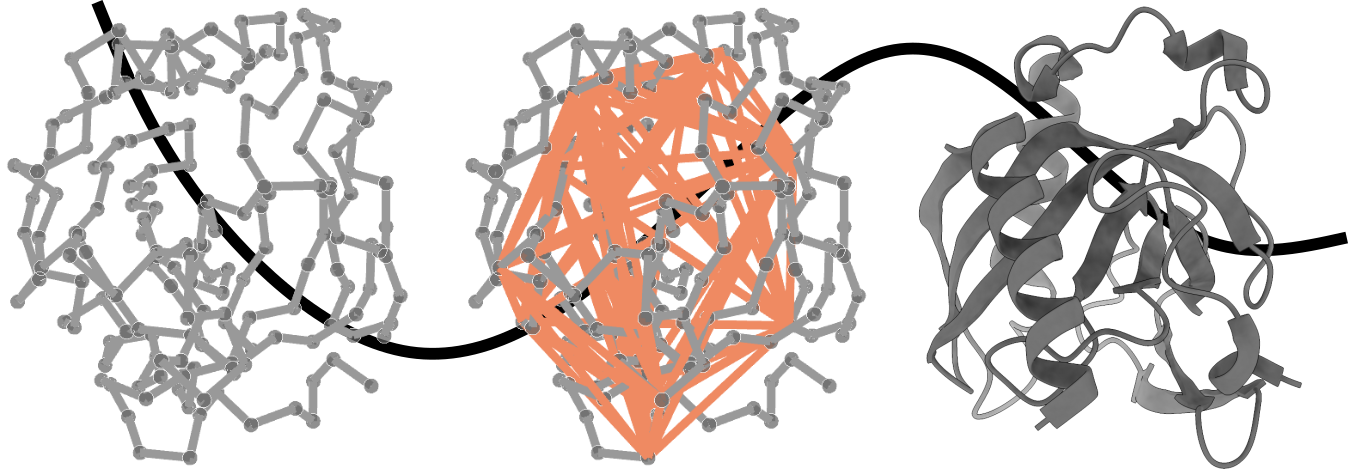
\includegraphics[]{Chapter.6/Figures/ch6.p%%ng}
%%    \vspace{0.25cm}
%%  \end{center}
%%}

\begin{flushleft}
  \vspace*{\fill}
  \rule{\textwidth}{1pt}\\[0cm]
  This chapter includes parts of the following publication:\\
  \textbf{A perspective towards mass-spectrometry-based \emph{de novo} sequencing of endogenous antibodies}\\
  \footnotesize
  \vspace{0.3cm}
  Sebastiaan C. de Graaf*, Max Hoek*, Sem Tamara and Albert J.R. Heck \\
  %%\vspace{0.3cm}
  \textbf{\emph{mAbs}} (2021), 14:1, 2079449, DOI: 10.1080/19420862.2022.2079449 \emph{Review}\\
  %%\footnotesize
  \vspace{0.3cm}

  \textsuperscript{*} These authors contributed equally to this work

\end{flushleft}

\newpage
\thumbforchapter

\section{Summary}
\lettrine[lraise=0.1, nindent=0em, slope=-.5em]{A}{ntibodies} are essential to adaptive immunity and represent one of the most polymorphic proteins found in the human body. This polymorphism provides the incredible flexibility seen in adaptive immunity and makes antibodies a true "personalized proteome", unique to each individual and adapted to their needs. However, this diversity also makes studying antibodies difficult. The chapters in this thesis detail efforts to develop generalizable data analysis strategies for studying secreted antibody repertoires using mass spectrometry.
\bigskip\\
\textbf{Chapter 2} is on a distinctive topic, as we highlight the importance of having generalized computational tools to effectively analyze large and complex cross-linking proteomic datasets. While crosslinking MS has emerged as an attractive method to probe protein interactions, the complexity of dealing with protein interactions rather than individual proteins has resulted in the production of large amounts of data, making processing difficult, especially for experiments targeting the whole proteome. To address this issue, we developed a tool that is interactive and facilitates analysis and visualization of these large datasets. The tool directly handles the output of XlinkX for Proteome Discoverer but can also be used with output from other platforms through a user-controllable text-file importer. It comes equipped with a spectrum viewer and supports preprocessing of replicate datasets, enabling easy handling of large amounts of data. We have also integrated data from protein databases Eggnog and Uniprot, which enable integrated gene ontology enrichment analysis, grouping based on function, and mapping of known post-translational modification sites, domains, and secondary structures. Another feature is length-based validation of detected crosslinks by mapping the crosslinked peptides onto validated structural models of proteins or protein complexes. In situations where no structure is available, structures obtained by homology modelling can be used. In such cases, crosslinked peptides are aligned to the homologous sequence to obtain a confident placement of the linked residues before the distance between these residues is calculated using the 3D structure. Crosslinks between two proteins with known structures where no structure of the complex is available can also be directly submitted to DisVis for visualization and quantification of the information content of distance restraints.
\bigskip\\
In \textbf{Chapter 3}, we show how advancements in intact protein mass spectrometry allow for the detection of IgG1 molecules in human serum with clonal resolution. This enabled the construction of personalized IgG1 repertoires. Despite there being an enormous number of theoretically possible clones, the observed antibody repertoires were relatively simple, with only several hundred clones dominating at any given time point. Moreover, while the majority of the clones in these profiles were stable over time, we observed substantial changes in the repertoires following a sepsis episode. We also demonstrated that a combination of peptide- and protein-centric mass spectrometry could be employed to \emph{de novo} sequence individual clones directly from the serum. The peptide-centric approach provided extensive coverage, while the protein-centric (fragmentation) approach provided sequence information that is inherently grouped per clone. The synergy between these techniques was used to sequence a single highly abundant clone from the sample of one of our donors.
\bigskip\\
\textbf{Chapter 4} showcases the potential of antibody repertoire profiling data to compare and characterize individual donors within a group. We constructed SIgA1 profiles for a cohort of six lactating women who had received two identical SARS-CoV-2 vaccinations. The resulting profiles complement findings from earlier ELISA-based titer level analysis of these samples, where a biphasic rise in spike-specific IgA was found. Our observations indicate the emergence of a heterogeneous polyclonal population of between 100 and 200 novel clones in all donors after vaccination. This vaccine-induced population is dominated by a persistent population of clones that appear shortly after the initial vaccination and persist until at least five days after the second. However, we also detect a population of clones that emerge more than three days after the second vaccination was administered, in every donor. In-depth analysis of a strong responder, selected by ELISA and confirmed by our data, reveals that the second rise in spike-specific IgA coincides with an abundant second dose-induced population, highlighting the divergent clonal makeup of what initially seemed like a symmetrical biphasic response. Additionally, we observed several highly abundant clones appear and subsequently disappear from the secreted repertoire over the course of $\sim$40 days, showing that highly abundant clones do not necessarily persist over time.
\bigskip\\
In \textbf{Chapter 5}, we built further upon the proof of concept for \emph{de novo} sequencing of endogenous antibodies by mass spectrometry initially presented in Chapter 3 to create a more standardized and broadly applicable workflow for sequencing antibody chains in mixtures using a combination of peptide- and protein-centric mass spectrometry. The proposed approach sequences a target chain in a modular, three-stage process based on germline domains. It starts with sequencing the framework regions, followed by complementarity determining regions with flanking framework regions, and ultimately full chain sequences. Through integration of middle-down fragmentation, we could resolve ambiguity in \emph{de novo} sequence predictions for the hypervariable complementarity determining regions. To achieve this, we filtered candidate sequences by comparing their theoretical mass to the gap between adjacent framework regions. We demonstrated the effectiveness of this approach by accurately sequencing a single targeted chain in a pure monoclonal antibody sample, an equimolar mixture of three monoclonal antibodies, and a polyclonal serum sample. This approach provides a broadly applicable workflow that could be used in future studies to sequence complex samples with high accuracy, as well as a step towards full automation of the process.\\
\clearpage

\section{Perspective and Outlook}
Recent work by Wolf et al. \cite{wolf2022antibody} demonstrated that an individual's antibody titers are a poor marker of the frequency of memory B cells generated following SARS-CoV-2, seasonal influenza, or EBV infection. If assessing humoral immunity through polyclonal antibody titers does not reflect an individual's ability to mount an antibody response, we need to find additional ways to determine an individual's level of protection. The research presented in this thesis describes a promising new strategy to achieve this goal through antibody repertoire characterization by using mass spectrometry.
By monitoring antibody dynamics at an unprecedented resolution, we can gain new insights into humoral immune responses by uncovering when, how, and why specific antibodies are generated in response to physiological events. Coupled with targeted sequencing of endogenous antibodies by MS, this approach holds exciting potential for drug discovery as integration of these techniques into therapeutic development pipelines could lead to significant advancements in the field. Moreover, large scale profiling of endogenous secreted antibody repertoires may lead to the definition of immune signatures for use in disease risk assessment, diagnostic classification, or measuring treatment effectiveness.

\subsection{The importance of standardized tools}
The advancements made over the last decade in MS-based antibody sequencing provide an optimistic outlook for the future. I expect that a therapeutic antibody discovered by MS could be right around the corner. Looking back at the timeline of key developments in the field of antibody sequencing, we can notice several clear trends (\textbf{\autoref{fig:fig6.1}}). Since the 1960s, rudimentary sample preparation for antibodies was available, but practical methods of obtaining sequence information appeared only in 1993, when Sanger sequencing was first applied to B cells. The first therapeutic antibody was registered in 1986, and this advent launched large-scale development of mAbs, with a hundred mAbs registered by 2008 \cite{raybould2020thera-sabdab:}. At that point, next-generation sequencing led to high-throughput sequencing workflows and further facilitated the lead-finding and development of therapeutic antibodies. Over the last 20 years, the rapid expansion of genome-based sequencing techniques kick-started antibody discovery by allowing large-scale BCR sequencing, and the number of deposited antibody sequences and registered antibody therapeutics has been growing exponentially ever since, with the 100\textsuperscript{th} therapeutic mAb being approved by the United States Food and Drug Administration (FDA) in 2021 \cite{mullard2021fda}. Observing this trend, the popularization of MS-based proteomics has now spurred the development of platforms for \emph{de novo} sequencing of antibodies heavily supported by MS, and I envision that the ongoing advancement of MS based antibody profiling and \emph{de novo} sequencing will complement available strategies by protein-level analysis. More specifically, monitoring of antibody repertoires could be used to select a limited number of reactive antibodies from a patient with an effective immune response, which could then be sequenced, recombinantly produced and screened for neutralizing capacity. Such a direct approach to antibody discovery would be much more straightforward than screening of B-cells at the DNA/RNA level.
\begin{figure*}[!htb]
  \center
  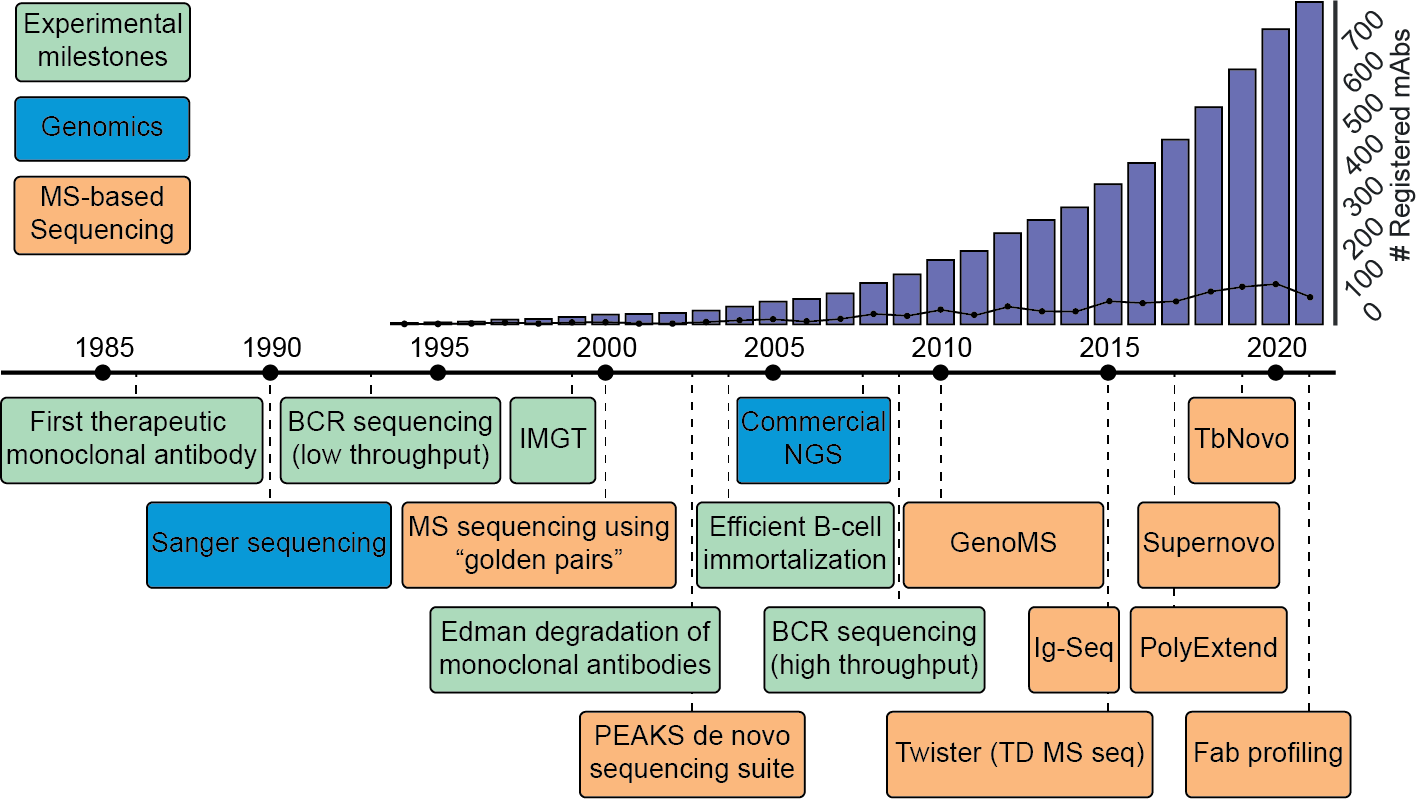
\includegraphics[]{Chapter.1/Figures/f7.png}
  \caption{\textbf{Timeline of key developments paving the way towards MS-based \emph{de novo} sequencing of serum antibodies.} Blue: Key developments in the field of genomic sequencing. Green: Key advances in the field of antibody research. Orange: Selected hallmark papers in the field of MS-based antibody sequencing. To visualize the impact of therapeutic antibody development, the bar graph indicates the cumulative number of registered antibody-based drugs, and the line shows the number of registrations for a given year \cite{raybould2020thera-sabdab:}.}
  \label{fig:fig6.1}
\end{figure*}
The impact of accessible, standardized, high throughput analytical methods, can be observed in the discovery of genomic and proteomic biomarkers as well \cite{simon2011genomic, cui2022high-throughput}. As standardized, high-throughput genomic and proteomic techniques became widely accessible, the number of genomic and proteomic biomarkers for disease risk assessment, early diagnosis, diagnostic classification and measuring treatment effectiveness rose drastically. I believe the current advances in immune response characterization could represent a similar opportunity, as large-scale, in-depth characterization of proteomic antibody repertoires may lead to the discovery of defined immune signatures that could be used as immunological biomarkers in very similar ways.

\subsection{Challenges}

\subsubsection{Larger sample size needed}
However, several challenges must be overcome before we can realize these goals. At the present time, there is, at the protein level, simply not enough antibody repertoire data to draw generalizable conclusions about antibody repertoire dynamics. While we clearly observe drastic changes in the clonal abundance profiles in response to disease and vaccination, the significance of these clones in relation to the antigen is not yet immediately apparent. The fact that these repertoires are unique to each donor means we cannot simply compare the clonal repertoires of donors to screen for antibodies of interest, which, combined with the complex and heterogenous nature of these responses, makes finding patterns extremely challenging. Larger cohorts will need to be studied, and the obtained longitudinal antibody repertoires should be correlated to established techniques. Existing techniques like ELISA, BCR sequencing and neutralization assays will be well complemented by the detailed characterization of the antibody repertoire. B cell receptor sequencing data could be used to determine the genetic and cellular origin of circulating clones, shedding light on whether novel clones are the result of somatic hypermutation or if they are the result of a completely new recombination of variable, diversity and joining (VDJ) gene recombination. Neutralization and binding assays could be used to determine exactly when an effective response emerges which can then be related to changes in the clonal profile. Such information on (individual) Fabs and the B-cells which produce them could be useful in studying the personalized nature of immune responses. As we increasingly correlate other assays to LC-MS Fab profiling data, we may also be able to distill a set of features common to effective neutralizing antibodies.

\subsubsection{Dealing with other isotypes and subclasses of antibodies}
A complete characterization of the antibody repertoire also requires including more antibody isotypes and subclasses, such as IgG1-4, IgA1-2, IgM, IgD, and IgE, as they each exhibit a specific tissue distribution and effectiveness against certain pathogens. Upon encountering antigens, B cells produce specific immunoglobulin isotypes and subclasses, depending on the antigen type and entry mode. In humans, IgG1 and IgG3 are effective against viruses, IgG2 against encapsulated bacteria, IgG4 and IgE against large extracellular parasites, and IgA1 and IgA2 against pathogenic bacteria at mucosal sites \cite{vidarsson2014igg, xu2012immunoglobulin}. As these subclasses target different antigens, it follows that their fab repertoires would not completely overlap. However, while differences between antibody isotypes and subclasses have been described extensively, comparatively little is known about their Fab repertoires. By comparing these repertoires we may gain a better understanding of the interplay between them.
The current Fab profiling methodologies for antibody characterization by mass spectrometry are focused on the two most abundant subclasses in humans, IgG1 and IgA1, as they require highly specific Fab-cleaving proteases that are only available for these subclasses. However, with the increasing demand for proteomic antibody characterization, it is likely that additional proteases will be developed, enabling the study of Fab repertoires of less abundant immunoglobulin isotypes and subclasses, thereby leading to a more complete understanding of the humoral immune response.

\subsubsection{Dealing with low-abundant clones}
A deep characterization of the proteomic antibody repertoire would also be highly desirable, as long lived, protective clones may not be among the most abundant fraction of the repertoire. While the observed proteomic repertoires were simple, consisting of 50-500 clones and dominated by a few abundant clones, the dynamic range of these secreted antibodies was wide and there may still be low abundant clones at concentrations below the current limit of detection. This is compounded by the fact that obtaining accurate uncharged, deisotoped masses for intact proteins (i.e. deconvolution) is an incredibly challenging task, particularly for low abundant species in complex samples. As we identify clones by mass and retention time, inconsistent mass determination impedes our ability to perform longitudinal tracking of clones in question and can lead to an underestimation of clonal longevity and an inability to deconvolute the LC-MS signal of a clone to an “antibody-like” Fab mass (i.e., a mass of 45-53 kDa) will result in failure to identify said clone. Similarly, a robust chromatography setup is required to prevent shifts in retention time due to an unstable system.

\subsubsection{Clonal lineage analysis and profiling MS}
Outside of experimental variation or artefacts of spectral processing, antibodies are highly polymorphic species and as such are subject to constant mutations which almost certainly lead to significant mass- and retention time shifts. Mutated clones would therefore show up as novel species in the antibody repertoire. While the ability to distinguish between these clones makes our analysis powerful, it also means that we are unable to identify clones with a shared clonal ancestor. While such clonal lineage analysis should in theory be greatly facilitated by referring detected masses to BCR-sequencing data, we have only observed a very small overlap between these two data streams. This apparent disjoint between the genomic or transcriptomic BCR sequences and proteomic data suggests that we are still missing a piece of the puzzle. A possible explanation lies in the sampling of the sequenced B cells. The most commonly used source of B cells for BCR sequencing is peripheral blood mononuclear cells, which only represent about 2\% of the total B cell population \cite{guthals2017de}.

\subsubsection{The need for full sequencing}
While limited sequence information, in the form of sequence tags for example \cite{tabb2008directag:}, can be used to reject the possibility of a shared clonal lineage, complete certainty requires full knowledge of the protein sequence of two clones. Unfortunately, in the current stage of implementation, \emph{de novo} sequencing of antibodies is not suitable for such analysis or at least not at a significant scale, as it is still a highly challenging task which requires manual curation by experts to derive the correct sequence. This manual curation is not only time-consuming, but also makes the process subject to interpretation errors when compared to more established sequencing techniques such as next generation DNA/RNA sequencing. As such, the need for automation is high, to improve not only the throughput but also the reproducibility and robustness.

\subsubsection{Sequencing-specific challenges}
Several challenges need to be overcome to achieve automated sequencing of abundant clones in polyclonal mixtures. Similar to deconvolution of intact mass spectra (MS1), accurate and consistent deconvolution of fragmentation spectra (MS2) is immensely challenging, doubly so as signal intensity is split across multiple fragments. Low abundant fragments are difficulty to acquire, and fragment coverage (i.e. the fraction of amide bonds that have one or more matching fragment mass in the spectrum) is typically limited \cite{he2018protein}. Peptide-centric analysis are hindered by the presence of other clones with homologous sequences, short peptide length and low depth of coverage, which make read assembly exceptionally challenging. Nevertheless, leveraging the synergy between the peptide- and protein-centric MS, as well as the available germline sequences has made sequencing of abundant clones in serum possible, and the generalizable workflow presented in this thesis can be used as a steppingstone towards full automation.

\subsubsection{Factors impacting sequencing strategies}
As antibody samples can be incredibly diverse, a big challenge for a robust antibody sequencing workflow is keeping the workflow broadly applicable. The optimal strategy for a sequencing experiment depends on many factors: How many other clones are in the sample? Are these other clones relatively abundant compared to your target clone? Are specific proteases available to facilitate middle down analysis? How much sample is available? Are there coeluting clones? Is there the possibility for affinity purification or fractionation prior to sequencing? How divergent is the clone from the germline sequence? How good is bottom-up coverage? How good is top-down coverage? Many of these questions cannot be answered before starting the experiment or require additional experiments and therefore time, resources, and sample. While this may seem like a negative outlook, it is good to remember that just a few years ago detection and deconvolution of individual antibody clones in complex samples such as serum seemed practically impossible and sequencing even more so. The incredible advances in the field of biomolecular mass spectrometry over the past decades are an indication that there really is no telling how far we can still improve through incremental improvements, not only to spectral processing and acquisition but also to downstream processing of the data. In my opinion, the current stage of implementation of \emph{de novo} sequencing of endogenous antibodies has only scratched the surface of the possibilities, and there is a litany of opportunities to improve data analysis, instrumentation and protocol adaptations that are readily available.

\subsubsection{Protein centric improvements}
Nano-flow LC-MS can reduce sample requirements up to 100x, making it possible to acquire more middle down fragmentation data using the same sample. However, these systems are less robust than the high-flow systems used in our current experimental protocol \cite{wilm1996analytical, gatlin1998protein}. Parallel acquisition strategies as seen in several 2D-MS techniques could be used to boost signal intensity \cite{vasilopoulou2020trapped, ridgeway2018trapped, graham2023characterizing}, and super resolution methods could provide greater resolving power \cite{grinfeld2017phase-constrained}. Improving precursor selection for fragmentation either by implementing some form of real-time processing \cite{jeong2022flashida} or providing an inclusion list of target precursors based on a separate full MS spectrum of the same sample. Additionally, while the current generalized implementation uses fragmented reduced antibody chains, fragmentation of intact Fabs through ECD can yield highly complementary fragments which could be beneficial to the sequencing process \cite{boer2020selectivity}. Furthermore, additional fragmentation methods could be used to increase sequence coverage, as different fragmentation methods will preferentially fragment different backbone positions \cite{dupré2021de, brodbelt2016ion}. We have also landed on the Xtract and Respect deconvolution algorithms as our deconvolution method of choice, but there are alternatives out there. One drawback of our current methodology is that it is restricted to deconvolution of scans from a single raw file and does not allow for manual selection of MS2 scans to average for deconvolution, instead only supporting averaging scans over a selected retention time window. Ms\_deisotope \cite{klein2021mobiusklein/msdeisotope:} is one such alternative that could be explored.

\subsubsection{Peptide centric improvements}
Our peptide centric efforts have been centered around using the \emph{de novo} read assembly tool stitch \cite{schulte2022template-based}, combined with PEAKS \emph{de novo} sequencing suite \cite{ma2003peaks:}, both of which are under continued development along, as are \emph{de novo} peptide sequencing algorithms and are thus likely to show improved performance over time. While the employed peptide-centric experimental strategies are highly optimized through selection of complementary proteases and defining a robust data acquisition method \cite{peng2021mass}, we still find ways to improve throughput or performance regularly, for example through the use of SP3 beads \cite{johnston2022solvent}, and potential future improvements could include providing exclusion lists of known constant region peptides.

\subsection{Conclusion}
The work presented in this thesis emphasizes the need for advanced analytical strategies in studying antibody dynamics and showcases the potential of MS-based proteomics as one such strategy. In doing so, I hope to have made studying these complex molecules less daunting for future researchers by outlining analytical strategies for untangling them.
Historically, the complexity of antibodies has made them difficult to analyze on a large scale, as they lack the universal protein sequence databases used in other proteomic studies. However, recent advances in MS-based proteomics and \emph{de novo} sequencing have paved the way for their inclusion, as evidenced by the increasing number of published strategies for proteomic analysis of these repertoires. Combined with the immunological studies of unparalleled scale that we are seeing since the SARS-CoV-2 pandemic, the stage now looks to be set for large scale, in depth, proteomic analysis of endogenous antibody repertoires.
The incredible advances in studying these repertoires in multidisciplinary, collaborative studies has left me feeling highly optimistic about the future of this field. Through comprehensive analysis of endogenous antibody repertoires we can gain a deeper understanding of the immune responses they are a part of and I believe that mass spectrometry will play an integral role in untangling these personalized proteomes.
\begin{otherlanguage}{dutch}
  \clearpage


  \section{Samenvatting}
  Antilichamen zijn een essentieel onderdeel van ons immuun systeem en behoren tot de meest polymorfe eiwitten in het menselijk lichaam. Dit polymorfisme zorgt voor de ongelooflijke flexibiliteit van het verworven immuunsysteem en maakt ons antilichamen repertoire tot een "gepersonaliseerd proteoom", uniek voor elk individu en aangepast aan diens behoeften. Deze diversiteit maakt het analyseren van antilichamen echter ook zeer uitdagend. De hoofdstukken in dit proefschrift beschrijven mijn contributies aan het ontwikkelen van generaliseerbare computationale analyse strategieën voor het bestuderen van antilichaam repertoires met behulp van massaspectrometrie.
  \bigskip\\
  \textbf{Hoofdstuk 2} is uniek in dit proefschrift, omdat we het belang benadrukken van algemene computationele hulpmiddelen om grote en complexe crosslinking proteomics datasets effectief te analyseren. Crosslinking MS is een aantrekkelijke methode geworden om eiwitinteracties te onderzoeken, maar levert zeer grote datasets op, omdat de complexiteit van eiwitinteracties exponentieel stijgt ten opzichte van individuele eiwitten. Dit heeft geleid tot de productie van grote hoeveelheden complexe datasets waarvan interpretatie moeilijk is, vooral voor experimenten gericht op het gehele proteoom. Om dit probleem te verhelpen hebben wij een interactief programma ontwikkeld dat de analyse en visualisatie van deze grote datasets vergemakkelijkt. Het programma, CrossID, verwerkt de output van XlinkX voor Proteome Discoverer, maar kan ook worden gebruikt met output van andere platforms door een flexibele import-module. Het kan spectra annoteren en visualiseren en ondersteunt de analyse van replicaten, zodat grote hoeveelheden gegevens gemakkelijk kunnen worden verwerkt. We hebben ook gegevens geïntegreerd uit de Eggnog en Uniprot databases, die geïntegreerde genontologieverrijkingsanalyse, groepering op basis van eiwitfunctie, en visualisatie van bekende posttranslationele modificatieplaatsen, domeinen en secundaire structuren mogelijk maken. Een andere functie is validatie van gedetecteerde crosslinks middels hun lengte door het plaatsen van de gecrosslinkede peptiden op gevalideerde structurele modellen van eiwitten of eiwitcomplexen. In situaties waarin geen structuur beschikbaar is, kunnen structuren verkregen door homologiemodellering worden gebruikt. In dergelijke gevallen worden gecrosslinkede peptiden met behulp van sequentiealignering (Engels: sequence alignment) geplaatst op de homologe sequentie om een betrouwbare plaatsing van de gekoppelde residuen te verkrijgen waarna de afstand tussen deze residuen wordt berekend aan de hand van de 3D-structuur. Crosslinks tussen twee eiwitten met bekende structuren waar geen structuur van het complex beschikbaar is kunnen ook direct worden ingediend bij DisVis voor visualisatie en kwantificering van de informatie in de crosslinks. Hierbij worden de crosslinks, en het feit dat deze een bekende min- en maximum lengte hebben, gebruikt om een structuur te genereren die zo goed mogelijk overeenkomt met de crosslinking data.
  \bigskip\\
  In \textbf{hoofdstuk 3} laten we zien dat ontwikkelingen in eiwitmassaspectrometrie de detectie van individuele IgG1-moleculen in menselijk serum mogelijk maakt, met klonale resolutie. Dit stelde ons in staat om gepersonaliseerde klonale IgG1-repertoires te construeren. Deze serologische repertoires werden gedomineerd door enkele honderden klonen, een onverwachts laag aantal wanneer het enorme aantal theoretisch mogelijke klonen in acht wordt genomen. Bovendien waren deze profielen grotendeels stabiel: Het merendeel van de gedetecteerde klonen was langdurig aanwezig. We zagen echter ook aanzienlijke veranderingen in de repertoires na een sepsis-episode. Tevens hebben we aangetoond dat een combinatie van peptide- en eiwit-gerichte massaspectrometrie kan worden gebruikt om de sequentie van individuele klonen uit het serum \emph{de novo} te bepalen. De peptide-centrische benadering levert hierbij een uitgebreide dekking op, terwijl de eiwit-centrische benadering sequentie-informatie oplevert die per definitie gegroepeerd is per kloon. De synergie tussen deze technieken werd gebruikt om de sequentie van een enkele zeer abundante kloon uit het serum van een van onze donoren te bepalen.
  \bigskip\\
  \textbf{Hoofdstuk 4} beschrijft hoe wij de antilichaam repertoire-profileringstechniek uit Hoofdstuk 3 gebruikt hebben om individuele donoren binnen een groep te vergelijken en te karakteriseren. We hebben SIgA1-profielen samengesteld voor moedermelk van een cohort van zes moeders, die twee identieke SARS-CoV-2 vaccinaties hadden ontvangen. De betreffende profielen vormden een aanvulling op bevindingen van eerdere ELISA-gebaseerde analyse van deze monsters, waarbij een bifasische stijging van spike-specifiek IgA werd gevonden. In alle donoren detecteerden wij een heterogene polyklonale populatie van tussen de 100 en 200 klonen die na vaccinatie onstonden. Deze populatie werd gedomineerd door populatie van persistente klonen die kort na de eerste vaccinatie verschijnt en blijft bestaan tot ten minste vijf dagen na de tweede vaccinatie. Wij observeerden bij elke donor ook een populatie klonen die pas meer dan drie dagen na de tweede vaccinatie ontstaan. Diepgaande analyse van een sterke responder, geselecteerd door ELISA en bevestigd door onze analyse, toonde aan dat de tweede stijging van spike-specifiek IgA van deze donor werd gedreven door een zeer abundante populatie van door de tweede dosis geïnduceerde klonen, wat de uiteenlopende klonale samenstelling benadrukt van wat aanvankelijk leek op een symmetrische bifasische respons. Bovendien zagen we enkele zeer abundante klonen verschijnen en vervolgens verdwijnen uit het repertoire in een periode van $\sim$40 dagen, waaruit blijkt dat zeer overvloedige klonen niet noodzakelijk langdurig dominant blijven.
  \bigskip\\
  In \textbf{hoofdstuk 5} bouwen we op in hoofdstuk 3 gelegde funderingen voor antilichaam-sequentiebepaling, door een meer gestandaardiseerde en algemeen toepasbare computationele workflow te creëren voor de \emph{de novo} sequentiebepaling van antilichaamketens in mengsels met behulp van een combinatie van peptide- en eiwitgerichte massaspectrometrie. Onze aanpak bepaalt de sequentie van een geselecteerde eiwitketen in een modulair, drieledig proces op basis van sequentiedomeinen. We beginnen met het bepalen van de sequentie van de geconserveerde domeinen, de zogeheten “framework” regios. Vervolgens bepalen we de sequentie van de complementariteitsbepalende regios en de aangrenzende framework regios, voordat we uiteindelijk de sequentie van de volledige eiwitketen bepalen. Door het gebruik van middle-down fragmentatie konden we de ambiguïteit in de hypervariabele complementariteitsbepalende regios oplossen. Daartoe filterden wij kandidaat-sequenties door hun theoretische massa te vergelijken met het “gat” tussen de aangrenzende framework regios. We hebben de effectiviteit van deze aanpak aangetoond door de sequentie van een antilichaamketen te bepalen in drie monsters: Een zuiver monoklonaal antilichaammonster, een equimolair mengsel van drie monoklonale antilichamen en een polyklonaal serummonster. Deze aanpak biedt een generaliseerbare workflow die in toekomstige studies kan worden gebruikt om complexe monsters met hoge nauwkeurigheid te sequencen en brengt ons dichter bij volledige automatisering van dit proces.\\
\end{otherlanguage}


\clearpage
\section*{References}
\bibliographystyle{Stylesettings/pnas}
\patchcmd{\thebibliography}
{\clubpenalty 4000\widowpenalty 4000}
{\clubpenalties 1 10000 \widowpenalties 1 10000}
{}{}
\bibliography{chapmerge}
\stopthumb

